% 1987 年全国卷文科第 18 题：三棱锥及公垂线
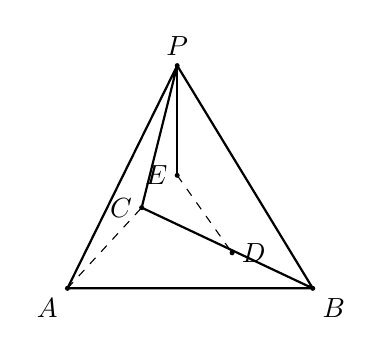
\begin{tikzpicture}[scale=0.82,>=stealth]
  \coordinate (P) at (1.7,3.45);
  \coordinate (A) at (0,0);
  \coordinate (B) at (3.8,0);
  \coordinate (C) at (1.15,1.25);
  \coordinate (E) at (1.7,1.75);
  \coordinate (D) at (2.55,0.55);
  \draw[thick] (P)--(A) (P)--(B) (P)--(C) (A)--(B) (B)--(C);
  \draw[dashed] (A)--(C) (E)--(D);
  \draw[thick] (E)--(P);
  \fill (P) circle (1.1pt) node[above] {$P$};
  \fill (A) circle (1.1pt) node[below left] {$A$};
  \fill (B) circle (1.1pt) node[below right] {$B$};
  \fill (C) circle (1.1pt) node[left] {$C$};
  \fill (E) circle (1.1pt) node[left] {$E$};
  \fill (D) circle (1.1pt) node[right] {$D$};
\end{tikzpicture}
